\setchapterpreamble[u]{%
    \margintoc\hfil%
    \dictum[Wethern's Law]{Assumption is the mother\\of all fuckups.}
}
\chapter{Results}
\labch{results}

The following sections look at the built spectrometer from a user's point of view. The first \refsec{user-perspective} describes the assembly and operation of the spectrometer built above. The following \refsec{water-signal} discusses how to measure a signal with water as a simple and approachable example.

\section{The spectrometer from a user's perspective}
\labsec{user-perspective}
The spectrometer was designed with ease of use and reconfigurability in mind. The individual parts are placed on separate boards, connected with standard \acrshort{sma} connectors. Broken parts can thus be easily exchanged. Old already existing parts can be used in conjunction with newly developed ones, facilitating the re-use of hardware and ensuring operation while a broken part is fixed or upgraded.

The software -- while still incomplete -- has the same goals as the hardware. It's written in \gls{python} with extensive documentation, comments throughout the code and accompanying guides to get started\sidenote{Take a look at the official \lstinline{README.md} in the \href{https://gitlab.ethz.ch/mstabel/nmr-spectrometer/-/tree/master/software/spectrometer}{official repository}}. Generally, the code tries to adhere to the ideas presented in \enquote{Uncle Bob's} book \textit{Clean Code} \sidecite{martinCleanCodeHandbook2008}.

\begin{marginfigure}
    \includesvg{images/logo_magnETHical.svg}
    \caption{Logo of the \textit{magnETHical} spectrometer project}
    \labfig{logo-magnethical}
\end{marginfigure}

There are five main parts to the spectrometer as explained in \nrefch{concepts}:
\begin{description}
    \item[The console] (i.e. the RedPitaya) responsible for sending, receiving and processing the \acrshort{rf} signals.
    \item[The power amplifiers] responsible for amplifying the signal generated by the console
    \item[The transmit-receive switch] responsible for switching between sending a signal into the probe from the transmit channel and receiving a signal back from the probe into the receive channel
    \item[The probe] consisting of the probe holder and the probe coil, responsible for emitting and receiving the \acrshort{rf} signal
    \item[The \acrlong{lna}s] responsible for amplifying the weak signal received by the probe before feeding it to the console for processing
\end{description}
The short conceptual overview is reproduced in figure \reffig{overview} for the reader's convenience. Each output needs to be connected to the input of the next device. The power connections are not shown in favour of clarity, but each part is labelled with the possible input voltages, in a range of \qtyrange{7}{15}{\volt}. For a more detailed description of the individual parts and their connections see the \enquote{magnETHical} project page (compare \reffig{logo-magnethical}) or the descriptions above.

\begin{figure*}[!htb]
    \centering
    \begin{circuitikz}[european]
        \ctikzset{bipoles/amp/width=0.9}
        \draw[nodes={align=center}]
        (0,0) coordinate(mid)

        % RP
        (mid) node[draw, align=center, minimum height=5.5cm, minimum width=2cm](redpitaya){Red\\Pitaya\\SDRlab\\122-16}
        ($(redpitaya.east)!0.75!(redpitaya.north east)$) coordinate(rptx) node[left]{TX\\(Out 1)}
        ($(redpitaya.east)!0.75!(redpitaya.south east)$) coordinate(rprx) node[left]{RX\\(In 1)}

        % TX
        (rptx) to[lowpass,l=SCLF-27+,>] ++(5,0)
        to[amp,t=\acrshort{pa},l=ADL5536\\PHA-202+,>] ++(5,0) coordinate(tx)

        % Circulator
        (mid -| tx) node[circulator,label={left:QPC6324}](circ){}
        (tx) -| (circ.n) node[inputarrow,rotate=270]{}

        % RX
        (rprx -| circ) coordinate(rx)
        (circ.s) |- (rx)
        (rx) to[amp,t=\acrshort{lna},l=PHA-13LN+,>] ++(-2.5,0)
        to[amp,t=\acrshort{lna},l=PHA-13LN+,>] ++(-2.5,0)
        to[amp,t=\acrshort{lna},l=PHA-13LN+,>] ++(-2.5,0)
        to[lowpass,l=SCLF-27+,>] ++(-2.5,0) node[inputarrow,rotate=180]{}

        % Probe
        (circ.e) -- ++(1,0)
        node[dinantenna](probe){}
        node[below=1ex]{3D-printed\\probe holder}
        ;
    \end{circuitikz}

    \caption{\captiontitle{Component overview.} The schematic contains all physical parts of the \acrshort{nmr} spectrometer that need to be connected through \acrshort{sma} cables.}
    \labfig{overview}
\end{figure*}

\subsection{Setting up the RedPitaya}
Having ordered or built the parts, connected them using \acrshort{sma} cables and powered them through a lab power supply, the console needs to be configured. The configuration of the console is relatively simple as most of the complexity has been programmed into the \gls{python} control library. The user thus only needs to ensure that a working \acrshort{linux} distribution is running on the \acrshort{rp} and that the \acrshort{ip} address is known. The official distribution that is pre-installed on the micro SD card that ships with the \acrshort{rp} is completely sufficient.

If the user needs to create a new microSD card, the \href{https://redpitaya.readthedocs.io/en/latest/quickStart/SDcard/SDcard.html}{setup of the microSD card is described in the \acrshort{rp} docs} and is summarized here for simplicity on a Linux based system.

\begin{enumerate}
    \item \href{https://redpitaya.readthedocs.io/en/latest/quickStart/SDcard/SDcard.html}{Download the newest microSD card image}
    \item Insert the microSD card into your computer.
    \item Figure out its name using \lstinline{lsblk} or \lstinline{df -h}, e.g. \lstinline{/dev/mmcblk0} or \lstinline{/dev/sdc}.
    \item Copy the image on the microSD card using\\ \lstinline{dd bs=1M if=red_pitaya_image_file.img of=/dev/mmcblk0 status=progress}
    \item Done!
\end{enumerate}

The \acrshort{rp} needs to be reachable through Ethernet from the computer running the control software. The easiest way is to connect them both to a \acrshort{dhcp} server\sidenote{An example for a \acrshort{dhcp} server would be any router or WiFi access point that automatically provides you internet access.} in the same network and lookup the IP address it got assigned by entering the name printed on it into a web browser. For a manual setup method for a direct connection in an isolated lab environment, see the \lstinline{README.md} in the control software repository or the \href{https://redpitaya.readthedocs.io/en/latest/quickStart/connect/connect.html#static-ip-configuration}{Static IP configuration guide in the RedPitaya documentation}\sidenote{For this document we assume the RedPitaya is reachable on the \acrshort{ip} \lstinline{192.168.1.100}}.

The control software needs to be able to remotely log in to the system through \acrfull{ssh}. For this, the \lstinline{sshd} server needs to be running, which is the case for almost any image you find -- including the official RedPitaya image\sidenote{The default username is \lstinline{root} and the default password is also \lstinline{root}. Sometimes there is no password -- in that case, just press \enquote{Enter} when asked for one. Remember nothing -- not even stars -- is displayed when typing the password}.

It is highly recommended to set up a passwordless login scheme from the computer to the \acrshort{rp}. Listing \ref{lst:pubkey} presents the necessary commands for creating a \lstinline{keyfile} and copying it to the \acrshort{rp} on a \acrshort{linux} machine. When asked, accept the recommended settings for the \lstinline{keyfile} -- don't set a password for it! Enter your password when prompted to do so.

\begin{listing}[h!bt]
    \begin{minted}{shell-session}
        $ ssh-keygen -t ed25519             # create a keyfile
        $ ssh-copy-id root@rp-xxxxxx.local  # alternatively: root@192.168.1.100
    \end{minted}
    \caption{Installing prerequisites}
    \label{lst:pubkey}
\end{listing}

\subsection{Setting up the control software}
On the computer, you need \href{https://git-scm.com/}{\lstinline{git}} and \href{https://www.python.org/}{\lstinline{python3}} to run the software. On Linux, they can usually be installed with one of the commands in Listing \ref{lst:install-prerequisites}.

\begin{listing}[h!bt]
    \begin{minted}{shell-session}
        $ dnf install python3 git   # (Fedora/RHEL/CentOS/...)
        $ apt install python3 git   # (Debian/Ubuntu/Mint/...)
        $ pacman -S python git      # (Arch/Manjaro/Artix/...)
    \end{minted}
    \caption{Installing prerequisites}
    \label{lst:install-prerequisites}
\end{listing}

With the prerequisites installed, the user can now install the spectrometer control software \gls{python} package. However, it is generally recommended to use \enquote{virtual environments}\sidenote{For more details see \href{https://peps.python.org/pep-0668/}{PEP 668} and \href{https://peps.python.org/pep-0405/}{PEP 405}} that create a new environment with packages and executables separate from the system and other programs. This functionality is already included in \gls{python}. Listing \ref{lst:setup} describes how to set up and activate a new \enquote{virtual environment} inside a \lstinline{~/spectrometer} folder.

\begin{listing}[h!bt]
    \begin{minted}{shell-session}
        $ cd ~
        $ mkdir spectrometer
        $ cd spectrometer
        $ python3 -m venv .venv
        $ source .venv/bin/activate    # Linux
        $ .venv/bin/activate.ps1       # Windows Powershell
        $ .venv/bin/activate.bat       # Windows Cmd
    \end{minted}
    \caption{Set up of a \enquote{virtual environment} (often called \enquote{venv}) in \gls{python}}
    \label{lst:setup}
\end{listing}

The user can now install the control software including all dependencies independently from the system they are working on using the commands in Listing \ref{lst:install}. The second one might take a while to run.

\begin{listing}[h!bt]
    \begin{minted}{shell-session}
        $ git clone https://gitlab.ethz.ch/mstabel/nmr-spectrometer
        $ python3 -m pip install ./nmr-spectrometer/software/spectrometer
    \end{minted}
    \caption{Installation of the python library with automated dependency resolution using \href{https://pypi.org/project/pip/}{\acrshort{pip}}. Assuming the user already installed and activated a virtual environment as described in Listing~\ref{lst:setup}.}
    \label{lst:install}
\end{listing}

The installation process automatically adds scripts for controlling the spectrometer to the command line. These can be used to manually set up the spectrometer hardware, flash the firmware and

\todo{Wassersignal Spannung (aus vergleich mit Funktionsgeneratorsignal). Vielleicht oben am Ende der Hardware?}

\section{Measuring a water signal}
With the above preparations, the system is ready to be used. The software and hardware support arbitrary pulse sequences with one transmit and one receive channel. The following presents the measurement results of different pulse sequences sent with the spectrometer and analysed with the control software.

While the significance of different parameters will be mentioned later in the text, and a short introduction has been presented in \refch{concepts}, a full introduction into \acrshort{nmr} is outside the scope of this text. For a better introduction than the author will ever be capable of, please take a look at other literature, such as \enquote{spin dynamics}\sidecite{levittSpinDynamicsBasics2008a} or \enquote{Experimental Pulse NMR}\sidecite{fukushimaExperimentalPulseNMR2019}. The following is a short recap to remind us of the necessary physical properties to be able to better appreciate the results.

Simply put, a nucleus of an \enquote{NMR active}\sidenote{For example \ch{^1H}, \ch{^{13}C}, \ch{^{19}F}, \ldots} atom will absorb and then later emit radio waves at a specific frequency that depends on an external magnetic field -- the stronger the field the higher the frequency:

\[
    \omega = \gamma{}B_0
\]

The specific frequency \(\omega\) is usually called the \emph{Larmor frequency}. \(\gamma\) is called the \emph{gyromagnetic ratio} and depends on the atom. Finally, \(B_0\) is the name for the external static magnetic field produced by a large magnet\sidenote{As opposed to \(B_1\) which is the magnetic component of the radio wave.}.

Nature now has it, that the exact frequency that the nuclei \emph{resonante} with depends on their surroundings. Inversely, we can thus exploit this property to figure out these surroundings if we know the frequency at which the nuclei resonate. \emph{Surroundings} include for example whether an atom is located next to another atom only in space due to some folding of a long molecule or whether a chemical bond is present as well.

Thus we need to send radio waves at multiple frequencies and then look at the corresponding return signals. To speed this process up, we can send all frequencies we're interested in at the same time using so-called \acrshort{ftnmr}.

\subsection{A first signal}

The simplest pulse sequence consist of a single excitation pulse intended to

\labsec{water-signal}
\begin{marginfigure}
    \centering
    \includesvg{simple_pulse_sequence.svg}
    \caption{\captiontitle{Simple pulse sequence} The usual depiction of a simple pulse sequence. The \enquote{RF pulse} is a high frequency \acrshort{rf} pulse close to the resonance frequency of the nuclei to be observed. After the pulse, a decaying sinus signal can be received on the same coil -  the so-called \acrfull{fid}.}
    \labfig{simple-pulse-sequence}
\end{marginfigure}

\begin{figure}[h!bt]
    \centering
    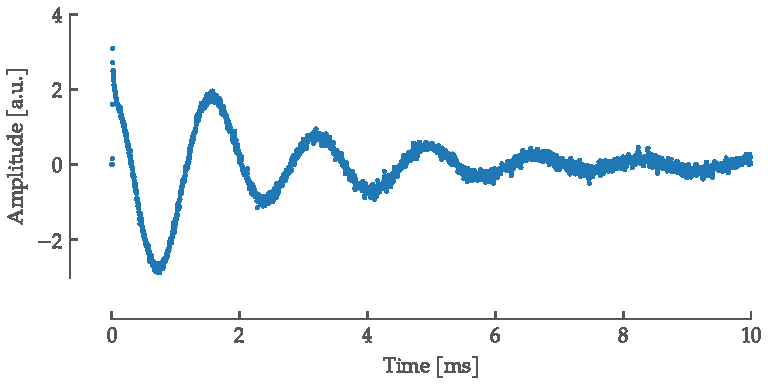
\includegraphics{fid_raw.pdf}
    \caption{\captiontitle{\acrfull{fid} of water.} The signal was recorded after a \qty{9}{\micro\second} impulse of a strength of \qty{1}{\watt} and a delay of \qty{25}{\micro\second}, waiting for the coil to ring down. \enquote{Andrew's probe} was used in this measurement with a transmit frequency of \qty{25.09}{\mega\hertz}}
    \labfig{fid-raw}
\end{figure}

\begin{figure}[h!bt]
    \centering
    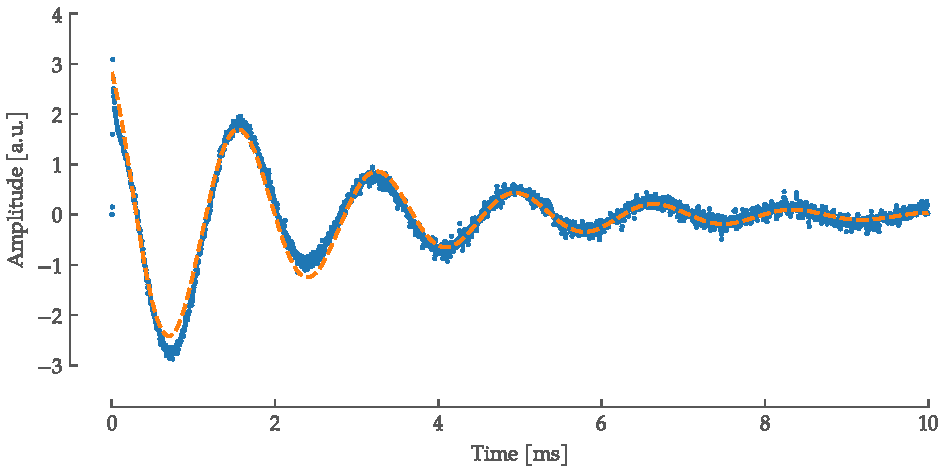
\includegraphics{fid_sine_fit.pdf}
    \caption{\captiontitle{\acrfull{fid} of water with a sine fit.} The blue data is the same as in \reffig{fid-raw}. The orange dashed line is the result of a least squares fit of a decaying sinus. It shows an exponential decay in amplitude with a $T_2^*$ of \qty{2.5}{ms} and a dominant frequency of about \qty{590}{\hertz}}
    \labfig{fid-sine-fit}
\end{figure}

\begin{figure}[h!bt]
    \centering
    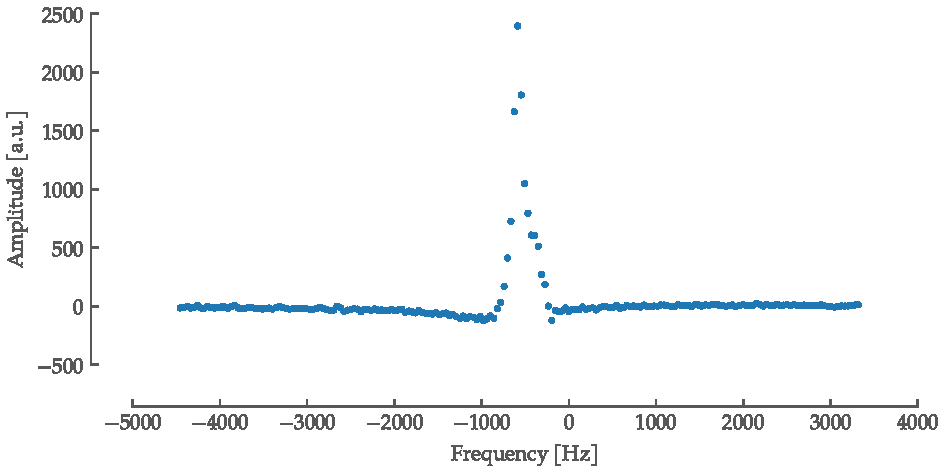
\includegraphics{fft_raw.pdf}
    \caption{\captiontitle{Fourier spectrum of \reffig{fid-raw}.} It shows a Lorentz-shaped peak around roughly \qty{600}{\hertz} with a slight broadening on the right side. The data was obtained through an automatic zero fill, complex Fouriertransform and an automated zero order phase correction of \ang{37}.}
    \labfig{fft-raw}
\end{figure}

\begin{figure}[h!bt]
    \centering
    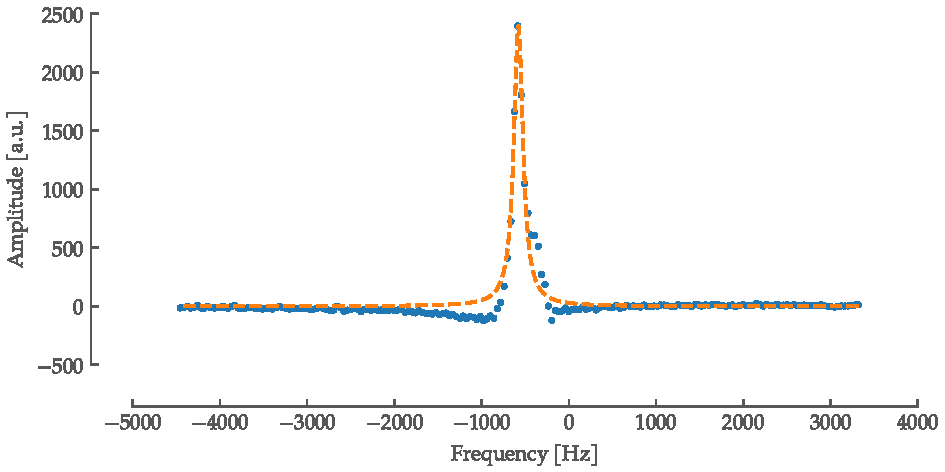
\includegraphics{fft_fit.pdf}
    \caption{\captiontitle{Fourier spectrum of \reffig{fid-raw} with lorentzian fit.} The Lorentzian curve was fit using a least-squares minimization approach. It's centred around \qty{-576}{\hertz} with a full width at half maximum of \qty{158}{\hertz}.}
    \labfig{fft-fit}
\end{figure}



\begin{figure}[h!bt]
    \centering
    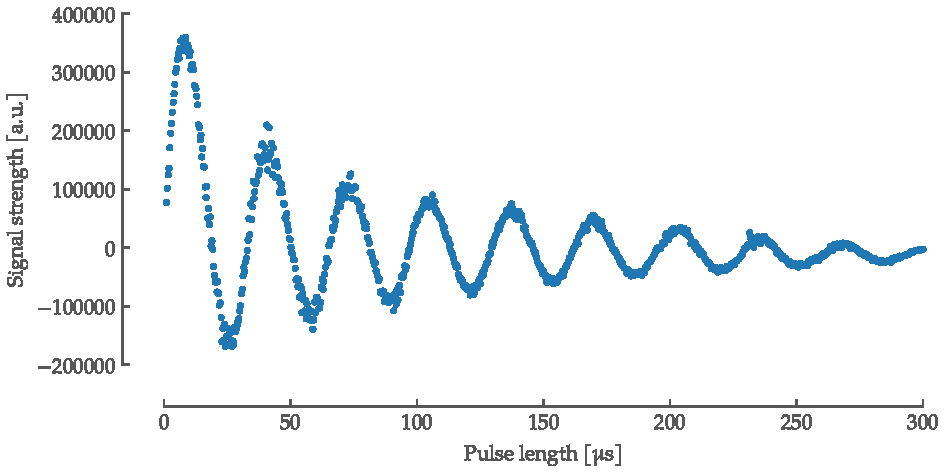
\includegraphics{rabi_nutation_raw.pdf}
    \caption{\captiontitle{Rabi nutation of the water signal}. Each data point was generated by performing an \acrshort{fid} experiment as described in \reffig{fid-raw} and integrating over the resulting peak (see \reffig{fft-raw}) to obtain a measure of signal strength. The phase correction applied to all points was identical.}
    \labfig{fft-fit}
\end{figure}

\begin{figure}[h!bt]
    \centering
    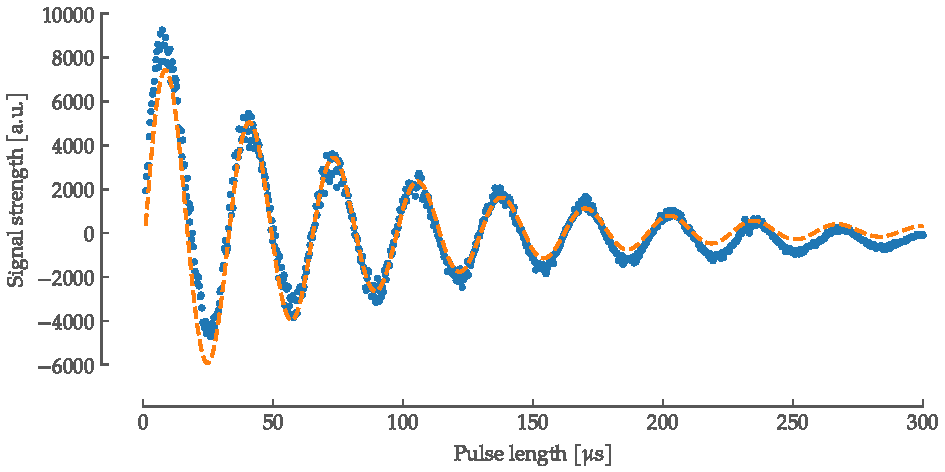
\includegraphics{rabi_nutation_fit.pdf}
    \caption{\captiontitle{Rabi nutation of the water signal with decaying sinus fit}. The data was fit using a least-squares approach to fit a decaying sinusoidal function. The fit has a period of \qty{32}{\micro\second}, giving the length of a $\frac{\pi}{2}$-pulse of \qty{8}{\micro\second}.}
    \labfig{fft-fit}
\end{figure}

\begin{marginfigure}
    \centering
    \includesvg{spin_echo_sequence_margin.svg}
    \caption{\captiontitle{Spin echo sequence}. A possible depiction of the spin echo sequence. A pulse of a duration that causes a \(\frac{\pi}{2}\) rotation of the spins and a pulse twice as long (i.e. length \(\pi\)) are applied with a delay of duration \(\tau\) in between. A spin echo is then observed with its peak after a delay of \(\tau\) after the second pulse.}
    \labfig{pulse-echo-sequence}
\end{marginfigure}

\begin{figure}[h!bt]
    \centering
    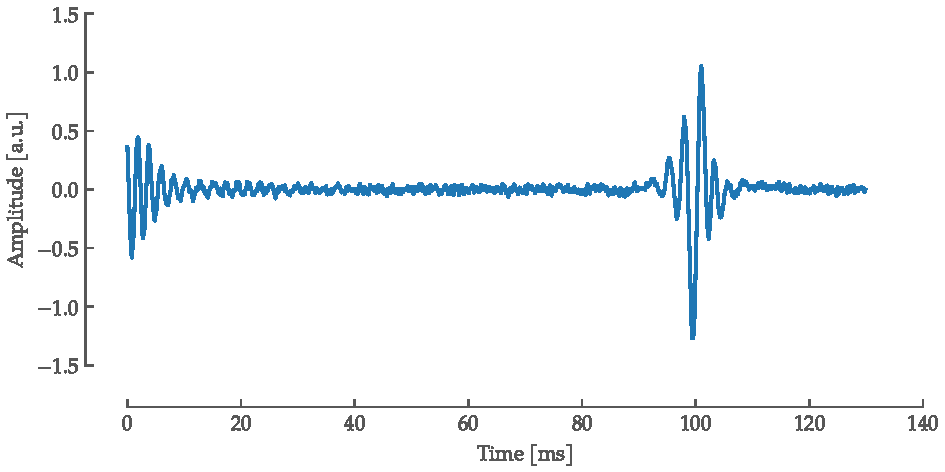
\includegraphics{spin_echo_avg.pdf}
    \caption{\captiontitle{Spin Echo}. Measurement of the received signal after the last pulse of a classic spin echo sequence (see \reffig{pulse-echo-sequence}). The \(\frac{\pi}{2}\) of \qty{9}{\micro\second} was sent with a power of \qty{1}{\watt}. The delay between pulses \(\tau\) was \qty{100}{\milli\second}. Data was recorded for \qty{130}{\milli\second} after the last pulse.}
    \labfig{spin-echo}
\end{figure}

\begin{marginfigure}
    \centering
    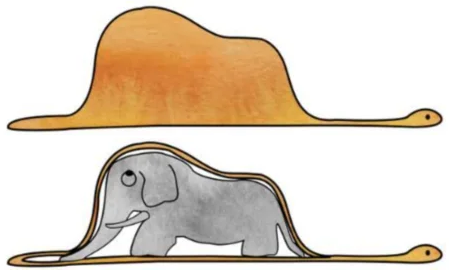
\includegraphics{little_prince_hat.png}
    \caption{\captiontitle{Le Petit Prince}. \enquote{My drawing was not a picture of a hat. It was a picture of a boa constrictor digesting an elephant.}\\
        --- Antoine de Saint-Exupéry}
    \labfig{pulse-echo-sequence}
\end{marginfigure}

\begin{figure}[h!bt]
    \centering
    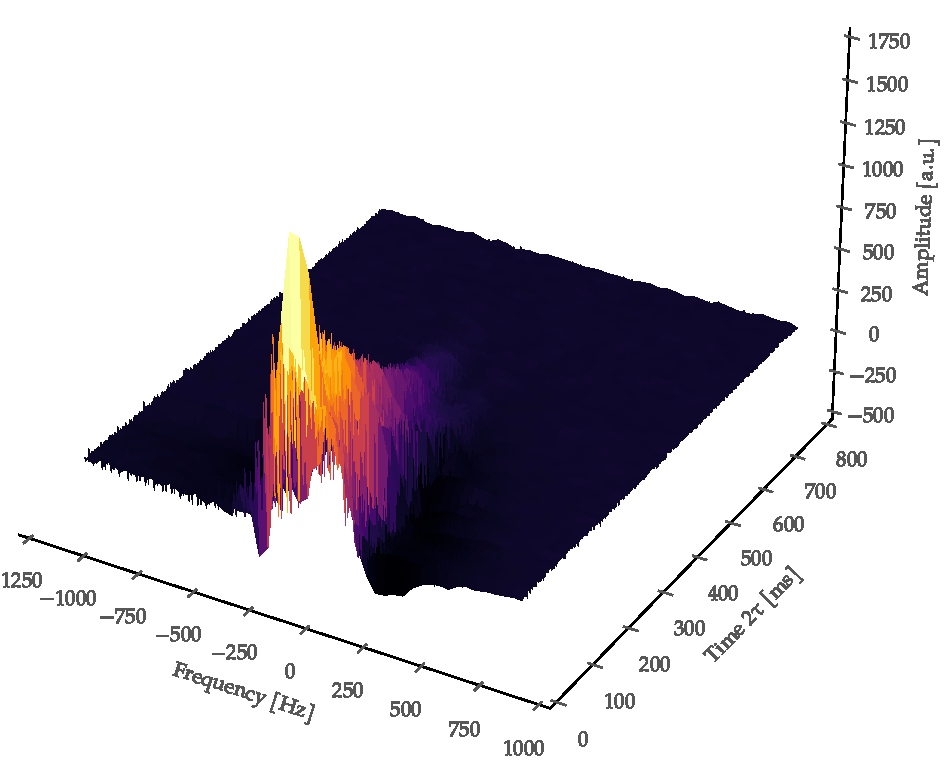
\includegraphics{t2_decay_3d_fft.pdf}
    \caption{\captiontitle{Fourier Transform of decaying spin echoes over delay length \(\tau\)}. The phase-corrected Fourier transforms are plotted in three dimensions over the delay \(\tau\) in between the pulses. The decay of the signal strength with increasing delay is clearly visible.}
    \labfig{t2-decay-3d}
\end{figure}

\begin{figure}[h!bt]
    \centering
    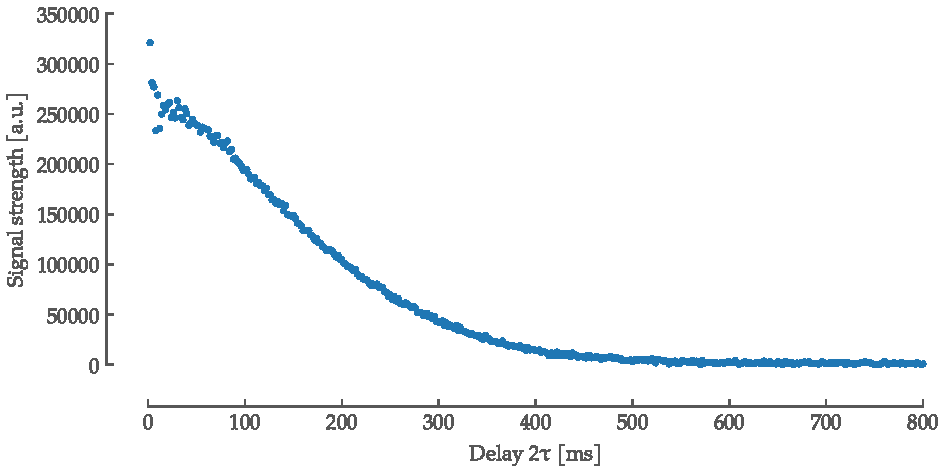
\includegraphics{t2_decay.pdf}
    \caption{\captiontitle{\(T_2\) decay of water}. Each data point is obtained by integrating the peak of the phase-corrected Fourier spectrum of a spin echo experiment as seen in \reffig{t2-decay-3d}. One can vaguely discern the expected exponential decay.}
    \labfig{t2-decay}
\end{figure}

\begin{figure}[h!bt]
    \centering
    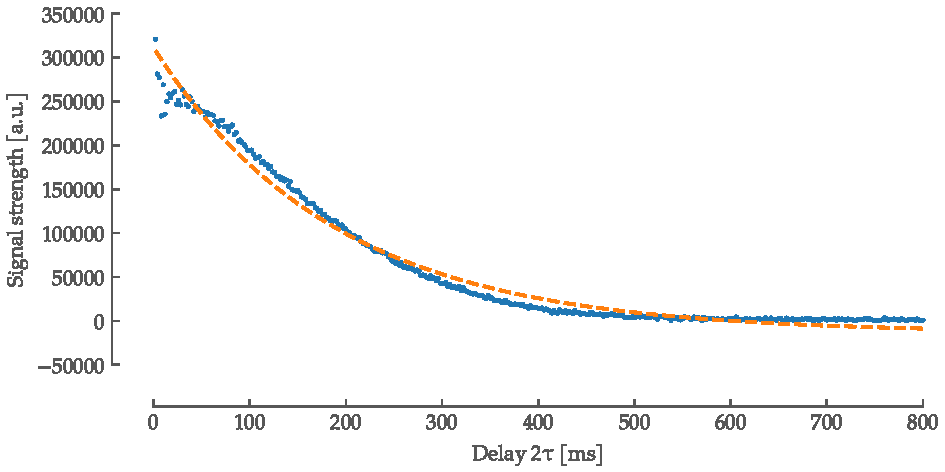
\includegraphics{t2_decay_fit.pdf}
    \caption{\captiontitle{\(T_2\) decay of water with an exponentially decaying function fitted}. The data points are the same as in \reffig{t2-decay}. The least-squares fit has a \(T_2\) decay time of \qty{190}{\milli\second}.}
    \labfig{t2-decay-fit}
\end{figure}

\section{Measuring a Toluene signal}
\labsec{toluol-signal}

\begin{marginfigure}
    \centering
    \includesvg[width=0.3\textwidth]{toluene.svg}
    \caption{\captiontitle{Chemical structure of Toluene.} Notice the two main components: The \ch{CH_3} methyl group on one side and the phenyl ring on the other. The hydrogen atoms in both have very distinct \acrshort{nmr} resonance frequencies and differ by about \qty{5}{\partspermillion}.}
    \labfig{pulse-echo-sequence}
\end{marginfigure}

\begin{figure}[h!bt]
    \centering
    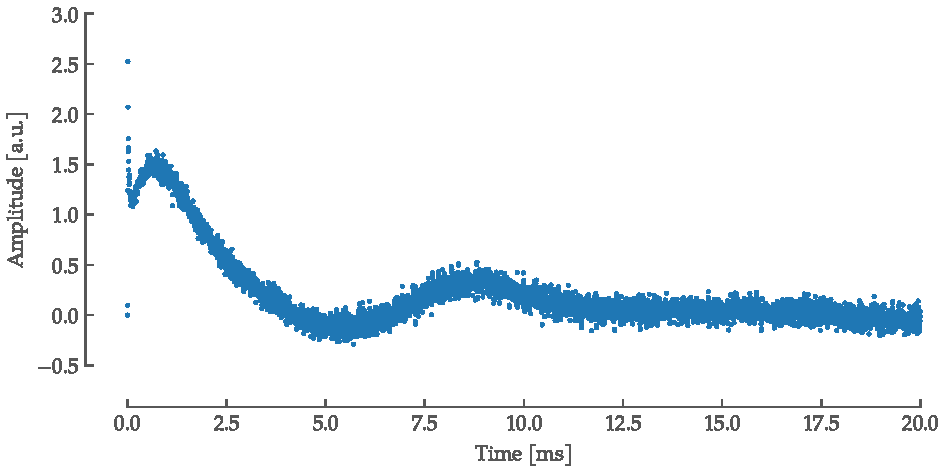
\includegraphics{fid_toluene.pdf}
    \caption{\captiontitle{\acrshort{fid} of Toluene}. It was recorded under similar conditions as the water above. A simple \(\frac{\pi}{2}\)-pulse of \qty{9}{\micro\second} with \qty{1}{\watt} power at \qty{25.0904}{\mega\hertz} was sent. After a delay of \qty{25}{\micro\second} the signal was recorded for \qty{20}{\milli\second}.}
    \labfig{fid-toluene}
\end{figure}

\begin{figure}[h!bt]
    \centering
    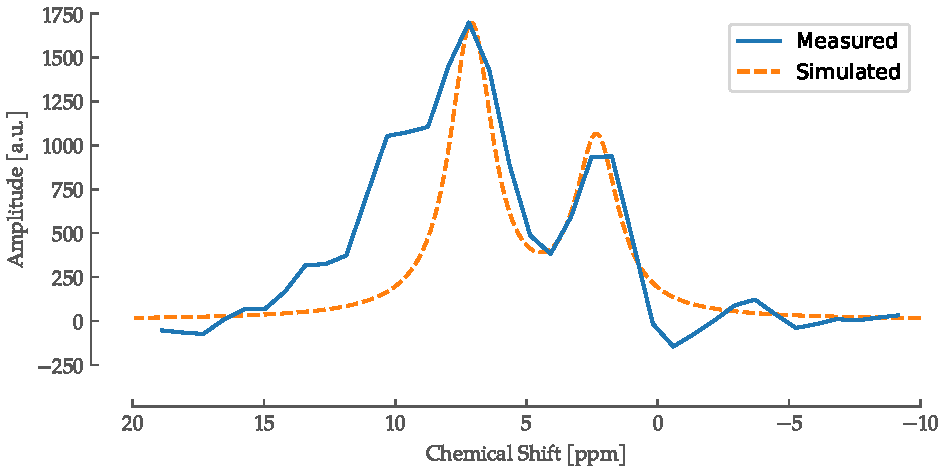
\includegraphics{fft_toluene.pdf}
    \caption{\captiontitle{\acrshort{fft} of Toluene measurement and simulation over a ppm scale}. The blue data line was obtained through a Fourier transform of the signal in \reffig{fid-toluene}. It was manually shifted by \qty{170}{\hertz} as there is no locking yet. The orange signal was created using MestReNova 14.3.3 simulating a spectra of Toluene at a $B_0$ field of \qty{25}{\mega\hertz}, a peak width of \qty{50}{\hertz} and scaled to match the measurement scale.}
    \labfig{fft-toluene}
\end{figure}